\section{理论分析}
\subsection{问题重述}
我们首先引入线性算子
\begin{align*}
&R:L^2(\Omega) \longrightarrow L^2(\Omega) \\
Ru(x,y)=&\int_\Omega K(x-x^1,y-y^1)u(x^1,y^1)dx^1dy^1
\end{align*}
其中 $K(x,\epsilon,y,\tau)$ 为脉冲响应函数,并且我们总假定线性算子 $R$ 是有界的。

若已知 $u$ 的模糊版本 $g$,则由方程 $g=Ru$ 求 $u$ 是一个典型的反问题,称为图像去模糊问题或图像去卷积\footnote{算子}。这里我们考虑含加性噪声的图像 $u_0$,含加性噪声的模糊图像 $u_0$ 满足方程
\[u_0=Ru+\eta\]
其中: $\eta$ 表示高斯白噪声,即
\[\int_\Omega \eta(x)=0,\int_\Omega \eta^2(x)=\sigma^2\]
综上所述,这里考虑的基本问题是:已知初值数据 $u_0$,算子 $R:L^2(\Omega) \longrightarrow L^2(\Omega)$ 是有界线性算子,图像噪声方差 $\sigma^2$,根据含噪声模糊图像模型
\[u_0=Ru+\eta\]
重建或者复原 $u$,特别的,当 $R$ 为恒同算子时,基本问题\footnote{什么}就称为去噪问题。

\subsection{问题分析}
以下我们考虑当 $R$ 为恒同算子时的去噪问题,即
\begin{equation}
u_0=u+\eta
\end{equation}
其中: $\eta$ 表示高斯白噪声,即
\begin{equation}
\label{zaosheng}
E\eta(x)=0,E\eta^2(x)=\sigma^2
\end{equation}
由噪声式 (\ref{zaosheng}) 的假设导致了两种约束
\begin{align}
\iint\limits_\Omega u(x,y)\,dx\,dy =\iint\limits_\Omega u_0(x,y)\,dx\,dy\\
\frac{1}{|\Omega|}\iint\limits_\Omega (u(x,y)-u_0(x,y))^2\,dx\,dy =\sigma^2
\end{align}
其中 $|\Omega|$ 为图像区域 $\Omega$ 的面积。

由Rudin、Osher 和Fatemi提出的 TV 图像复原模型,是图像复原中最成功的方法。与最小二乘复原模型相比,TV 模型最主要的差别是用梯度的 Ll 范数替代了它的 L2 范数,也就是最小化全变分(Rudin 认为,有噪声图像的全变分比无噪声图像的全变分明显大,最小化全变分可以消除噪声)。

令 $F_1(u)=\int_\Omega 2|\triangledown u|^{\frac{1}{2}}dxdy$,由于 $F_1(u)$ 具有平移不变性,即 $F_1(u+c)=F_1(u)$,$c$ 为任意常数,那么第一个约束实际上是自满足的。因此,通常我们只需要考虑第二个拟合约束。通过引入拉格朗日乘子 $\lambda$,可以定义一个新的能量泛函:
\begin{equation}
\label{nengliangfanhan}
J(u)=\int_\Omega 2|\triangledown u(x,y)|^{\frac{1}{2}} dxdy +\frac{\lambda}{2} \int_\Omega |u-u_0|^2dxdy
\end{equation}
其中,参数 $\lambda$ 对平衡去噪与平滑起重要作用。这是一个泛函求极值问题,即变分问题。

\subsection{PDE的推导}
从 (\ref{nengliangfanhan}) 式中可以看出该能量泛函为
\begin{equation}
J(u)=\int_\Omega F(x,y,u,\frac{\partial u}{\partial x},\frac{\partial u}{\partial y}) dxdy
\end{equation}
型泛函,其中
\begin{equation}
\label{Ffanhan}
F= 2|\triangledown u(x,y)|^{\frac{1}{2}}+\frac{\lambda}{2}|u-u_0|^2
\end{equation}
由泛函求极值的必要条件,有欧拉—拉格朗日方程(PDE)
\begin{equation}
\label{EL}
F_H-\frac{\partial}{\partial x}\{F_p\}-\frac{\partial}{\partial y}\{F_q\} =0
\end{equation}
其中 $p=\frac{\partial u}{\partial x},q=\frac{\partial u}{\partial y}$。所以对于 (\ref{Ffanhan})式有
\begin{equation}
F_H=\lambda(u-u_0),F_p=\frac{\frac{\partial u}{\partial x}}{|\triangledown u|^{\frac{3}{2}}},F_q=\frac{\frac{\partial u}{\partial y}}{|\triangledown u|^{\frac{3}{2}}}
\end{equation}
将上式代入式(\ref{EL}) 有:
\begin{align*}
\lambda (u-u_0)-\Big\{\frac{\partial}{\partial x}\Big\{\frac{\frac{\partial u}{\partial x}}{|\triangledown u|^{\frac{3}{2}}}\Big\}+\frac{\partial}{\partial y}\Big\{\frac{\frac{\partial u}{\partial x}}{|\triangledown u|^{\frac{3}{2}}}\Big\}\Big\}&=0 \\
\lambda (u-u_0)-\Big(\frac{\partial}{\partial x},\frac{\partial}{\partial y}\Big)\cdot \Big(\frac{\frac{\partial}{\partial x}}{|\triangledown u|^\frac{3}{2}},\frac{\frac{\partial}{\partial y}}{|\triangledown u|^\frac{3}{2}}\Big)&=0
\end{align*}
综上得到该模型的欧拉—拉格朗日方程(PDE):
\begin{equation}
\label{EL1}
-\triangledown \cdot (|\triangledown u|^{-\frac{3}{2}} \triangledown u)+\lambda (u-u_0)=0
\end{equation}
同理,对于能量泛函
\begin{equation}
J(u)=\int_\Omega \frac{1}{p}|\triangledown u(x,y)|^p dxdy +\frac{\lambda}{2} \int_\Omega |u-u_0|^2dxdy,0<p<2
\end{equation}
我们有对应的欧拉—拉格朗日方程(PDE):
\begin{equation}
-\triangledown \cdot (|\triangledown u|^{p-2} \triangledown u)+\lambda (u-u_0)=0
\end{equation}

\subsection{模型的数值实现}
通过前面的分析知道,求解变分问题式 (\ref{nengliangfanhan}) 与求解偏微分方程 (\ref{EL1})是等价的。我们在这里通过差分迭代法直接求解相关的平衡方程(稳定解)。

首先对图像进行等间隔采样,设采样步长 $h=1$。设目标像素为 $u(i,j),A=\big\{ (i,j+1),(i-1,j),(i,j-1),(i+1,j)\big\}$ 为目标像素 $u(i,j)$ 的四个邻域点位置的集合,如下图所示。$e,n,w,s$ 为对应的四个半像素点,它们不能直接从数字图像中得到。由于 $|\triangledown u|^{\frac{3}{2}}$ 出现在分母,为了避免它为零,我们引入一个小的正参数 $\epsilon$,使得$|\triangledown u|_\epsilon=\sqrt{\epsilon^2+|\triangledown u|^2}$。 只要保持 $\epsilon$ 足够小,便不会影响复原的性能。
\setlength{\unitlength}{0.8cm}
\begin{picture}(6,7.5)
\thicklines
\put(4,4.5){\circle*{0.2}}
\put(4,2.5){\circle*{0.2}}
\put(2,4.5){\circle*{0.2}}
\put(4,6.5){\circle*{0.2}}
\put(6,4.5){\circle*{0.2}}
\put(3,4.5){\circle*{0.2}}
\put(4,3.5){\circle*{0.2}}
\put(4,5.5){\circle*{0.2}}
\put(5,4.5){\circle*{0.2}}
\put(2,4.5){\line(1,0){4}}
\put(4,2.5){\line(0,1){4}}
\put(1,4.7){$(i-1,j)$}
\put(4,2){$(i,j-1)$}
\put(4.2,4.7){$(i,j)$}
\put(6.2,4.5){$(i+1,j)$}
\put(4,6.7){$(i,j+1)$}
\put(3,4.2){$w$}
\put(4.2,3.5){$s$}
\put(4.2,5.5){$n$}
\put(5,4.2){$e$}
\put(0.5,1){图1:目标像素 $(i,j)$ 与它的邻域}
\end{picture}

为了对式(\ref{EL1})进行数值实现,我们先令
\[v=(v^1,v^2)=\frac{\triangledown u}{|\triangledown u|_{\epsilon}^{\frac{3}{2}}}\]
那么旋度 $\triangledown \cdot$ 由差分表示为
\begin{equation}
\triangledown \cdot v=\frac{\partial v^1}{\partial x}+\frac{\partial v^2}{\partial y} \approx (v_e^1-v_w^1)+(v_n^2-v_s^2)
\end{equation}
下面给出 $v_e^1,v_w^1,v_n^2,v_s^2$ 的四个逼近:
\begin{align*}
v_e^1&=\frac{1}{|\triangledown u_e|_\epsilon^{\frac{3}{2}}}\Big[\frac{\partial u}{\partial x}\Big]_e \approx \frac{1}{|\triangledown u_e|_\epsilon^{\frac{3}{2}}} [u(i+1,j)-u(i,j)] \\
|\triangledown u_e|_\epsilon^{\frac{3}{2}}& \approx (\epsilon^2+[u(i+1,j)-u(i,j)]^2+[\frac{u(i+1,j+1)-u(i+1,j-1)}{2}]^2)^{\frac{3}{4}}
\end{align*}
同理可得:
\begin{align*}
v_w^1&=\frac{1}{|\triangledown u_w|_\epsilon^{\frac{3}{2}}}\Big[\frac{\partial u}{\partial x}\Big]_w \approx \frac{1}{|\triangledown u_w|_\epsilon^{\frac{3}{2}}} [u(i,j)-u(i-1,j)] \\
v_n^2&=\frac{1}{|\triangledown u_n|_\epsilon^{\frac{3}{2}}}\Big[\frac{\partial u}{\partial y}\Big]_n \approx \frac{1}{|\triangledown u_n|_\epsilon^{\frac{3}{2}}} [u(i,j+1)-u(i,j)] \\
v_s^2&=\frac{1}{|\triangledown u_s|_\epsilon^{\frac{3}{2}}}\Big[\frac{\partial u}{\partial y}\Big]_s \approx \frac{1}{|\triangledown u_s|_\epsilon^{\frac{3}{2}}} [u(i,j)-u(i,j-1)]
\end{align*}
所以有
\begin{equation}
-\triangledown \cdot (|\triangledown|^{-\frac{3}{2}} \triangledown u)=-\triangledown v=\sum_{q \in A}|\triangledown u_q|_\epsilon^{-\frac{3}{2}}[u(i,j)-u(q)]
\end{equation}
其中,我们定义
\begin{align}
\text{若}  q=(i-1,j),\text{则} p=(i-\frac{1}{2},j) \\
\text{若}  q=(i+1,j),\text{则} p=(i+\frac{1}{2},j) \\
\text{若}  q=(i,j-1),\text{则} p=(i,j-\frac{1}{2}) \\
\text{若}  q=(i,j+1),\text{则}  p=(i,j+\frac{1}{2})
\end{align}

因此式 (\ref{EL1})可转化为
\begin{equation}
\sum_{q \in A} |\triangledown u_p|_\epsilon^{-\frac{3}{2}}[u(i,j)-u(q)]+\lambda (i,j)[u(i,j)-u_0(i,j)]=0
\end{equation}
则可推出:
\begin{equation}
\label{ushi}
u(i,j)=\frac{\sum_{q \in A} |\triangledown u_p|_\epsilon^{-\frac{3}{2}}}{\lambda (i,j)+\sum_{q \in A} |\triangledown u_p|_\epsilon^{-\frac{3}{2}}}u(q)+\frac{\lambda (i,j)}{\lambda (i,j)+\sum_{q \in A} |\triangledown u_p|_\epsilon^{-\frac{3}{2}}}u_0(i,j)
\end{equation}
令
\begin{align}
\label{omega}
\omega_q&=\frac{1}{|\triangledown u_p|_\epsilon^{\frac{3}{2}}} \\
\label{hq}
h_q&=\frac{\omega_q}{\lambda (i,j)+\sum_{q \in A} \omega _q} \\
\label{h0}
h_0&=\frac{\lambda (i,j)}{\lambda (i,j)+\sum_{q \in A} \omega _q}
\end{align}
那么式(\ref{ushi})变为
\begin{equation}
u(i,j)=\sum_{q \in A}h_qu(q)+h_0u_0(i,j)
\end{equation}
其中
\begin{equation}
h_0+\sum_{q \in A}h_q=1
\end{equation}
采用 Gauss-Seidel 迭代法,在每一步 $n$:
\begin{equation}
\label{diedai}
u(i,j)^{(n)}=\sum_{q \in A}h_q^{(n-1)}u(q)^{(n-1)}+h_0^{(n-1)}u_0(i,j)
\end{equation}
综上有图像去噪的算法如下:
\begin{figure}[h]
\centering
\subfigure[$\lambda=\frac{1}{20^2}$]{\label{figure:1/20} 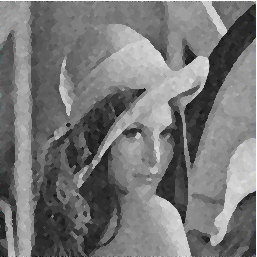
\includegraphics[width=0.4\textwidth]{003}}
\subfigure[$\lambda=\frac{5}{20^2}$]{\label{figure:5/20} 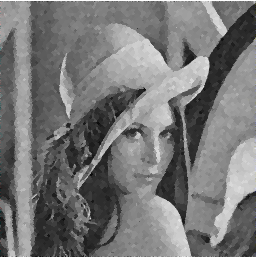
\includegraphics[width=0.4\textwidth]{004}}
\caption{第二章,第一组实验图}
\end{figure}
\begin{tabular}{|p{10cm}|}
\hline
初始化 $u^{(0)}$,通常取 $u^{(0)}=u_0$ ;\\
for $n=1,2,\cdots$  \\
 \quad for $i=1,2,\cdots,M$  \\
   \qquad for $j=1,2,\cdots,N$   \\
根据式 (\ref{omega}),(\ref{hq}),(\ref{h0})分别计算以 $(i,j)$ 为中心点的 $\omega_q,h_q,h_0$,然后利用
式 (\ref{diedai})计算 $u^{(n)}(i,j)$;\\
End \\
\quad End \\
    \qquad End \\
\hline
\end{tabular}